\documentclass[12pt,a4paper]{article}
\usepackage[utf8]{inputenc}
\usepackage[T1]{fontenc}


\renewcommand{\baselinestretch}{1}

\setlength{\hoffset}{-18pt}         
\setlength{\oddsidemargin}{0pt} % Marge gauche sur pages impaires
\setlength{\evensidemargin}{0pt} % Marge gauche sur pages paires
\setlength{\marginparwidth}{54pt} % Largeur de note dans la marge
\setlength{\textwidth}{481pt} % Largeur de la zone de texte (17cm)
\setlength{\voffset}{-18pt} % Bon pour DOS
\setlength{\marginparsep}{7pt} % Séparation de la marge
\setlength{\topmargin}{0pt} % Pas de marge en haut
\setlength{\headheight}{13pt} % Haut de page
\setlength{\headsep}{4pt} % Entre le haut de page et le texte
\setlength{\footskip}{27pt} % Bas de page + séparation
\setlength{\textheight}{720pt} % Hauteur de la zone de texte (25cm)
\setlength{\parindent}{0pt}
\setlength{\baselineskip}{15pt}

\usepackage{natbib}
\usepackage{graphicx}
\usepackage{amssymb}
\usepackage{amsmath} % Required for the align* environment
\usepackage{float}
\usepackage{pgfplots} 
\usepackage{algorithm}
\usepackage{algpseudocode} % test comment
\usepackage[hidelinks]{hyperref}
\usepackage{amssymb}
\usepackage{mathrsfs}
\pgfplotsset{compat=1.18}


\begin{document}
\title{SF1624 - Algebra och Geometri}
\author{Yunshan Luo}
\date{\today}
\maketitle
\newpage

\section{Linjära ekvationssystem och matriser}
\subsection{Determinant}
$2 \times 2$ matrisen
\[
A = \begin{bmatrix}
a & b \\
c & d
\end{bmatrix}
\]
\[
\implies det(A) = ad - bc
\]

$3 \times 3$ matrisen
\[
A = \begin{bmatrix}
a & b & c \\
d & e & f \\
g & h & i
\end{bmatrix}
\implies det(A) = aei + bfg + cdh - ceg - bdi - afh
\]

\begin{figure}[H]
    \centering
    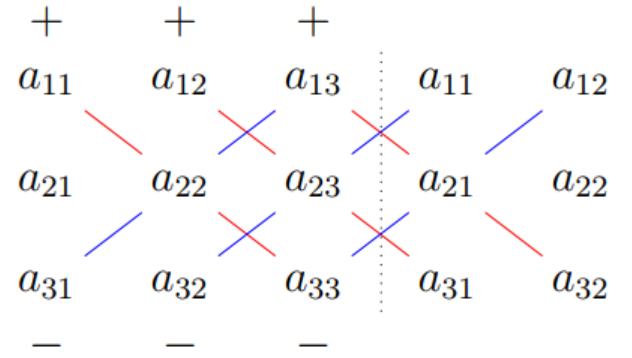
\includegraphics[width=0.35\textwidth]{sarrus.png}
\end{figure}

Determinant för en $n \times n$ matris kan beräknas med hjälp av \textbf{Laplaces kofaktorutveckling}
Kofaktorutveckla längs rad eller kolumn och håll rätt på tecknet enligt bilden
\begin{figure}[H]
    \centering
    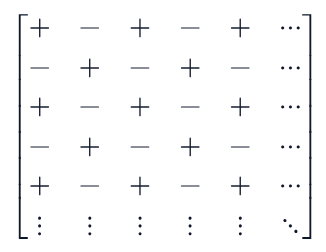
\includegraphics[width=0.35\textwidth]{laplace.png}
\end{figure}

\textbf{Populära genvägar}
\begin{enumerate}
    \item Om det finns \textbf{nollrad} eller \textbf{nollcolumn} är $det(A) = 0$
    \item Om matrisen är \textbf{triangulär} (eller \textbf{diagonal}) är $det(A)$ produkten av diagonalerna
\end{enumerate}

\textbf{Determinant och radoperatoiner}
\begin{enumerate}
    \item $B$ bildas från $A$ genom att byta plats på två rader
    \begin{itemize}
        \item $det(B) = -det(A)$
    \end{itemize}
    \item $B$ fås genom att addera en multipel av en rad till en annan rad i $A$
    \begin{itemize}
        \item $det(B) = det(A)$
    \end{itemize}
    \item $B$ fås genom att multiplicera en rad i $A$ med en konstant $k$
    \begin{itemize}
        \item $det(B) = k \cdot det(A)$
    \end{itemize}
    \item $det(A^T) = det(A)$
    \item $det(AB) = det(A) \cdot det(B)$
    \item $det(A^{-1}) = \frac{1}{det(A)}$
    \item $det(kA) = k^n \cdot det(A)$, där $n$ är dimensionen av matrisen
\end{enumerate}

\subsection{Gausseliminering}
\textbf{Totalmatris} exempel för ett linjärt ekvationssystem $Ax = b$:
\[
A = \begin{bmatrix}
    1 & 2 & 3 \\
5 & 6 & 7 \\
9 & 10 & 11 
\end{bmatrix}, \quad
b = \begin{bmatrix}
    4 \\
8 \\
12
\end{bmatrix}
\]
\[\implies
[A|b] =
\begin{bmatrix}
1 & 2 & 3 & | & 4 \\
5 & 6 & 7 & | & 8 \\
9 & 10 & 11 & | & 12
\end{bmatrix}
\]
\textbf{Trappstegsform} exempel:
\[
\begin{bmatrix}
1 & 2 & 3 & | & 4 \\
0 & -4 & -8 & | & -12 \\
0 & 0 & 0 & | & 0
\end{bmatrix}
\]
\textbf{Reducerade trappstegsform} exempel:
\[
\begin{bmatrix}
1 & 0 & 0 & | & 2 \\
0 & 1 & 0 & | & 3 \\
0 & 0 & 1 & | & 4
\end{bmatrix}
\]
\textbf{Fri variabel:} Variabel som kan anta arbiträra värden i tentor.

\subsection{Lösningsmängd}
Lösningsmängd är vektorrummet som uppfyller villkoret $Ax = b$ 
\vspace{10pt}
\begin{itemize}
    \item \textbf{Delrum:} Ett kontinuerligt rum som passerar origo
    \item \textbf{Homogent system} $Ax = 0$: Lösningsmängden är ett delrum av vektorrummet, kallat nollrummet.
    \item \textbf{Icke-homogent system} $Ax = b,\hspace{10pt} b \neq 0$: Lösningsmängden är en affint delrum av vektorrummet (förskjutning av nollrummet), kallat lösningsmängden.
\end{itemize}
\textbf{Dimensionssatsen:}
Givet att $A$ är en $m \times n$ matris med rang $r$, då gäller:
\[
\text{dim}(\text{lösningsmängden}) = n - r
\]

\subsection{Matrisinvers och inverterbarhet}






\end{document}